\section{Results and Analysis}\label{sec:results}

This section presents our experimental results across four dimensions: structured workload parity, the irregular workload performance gap, CUDA technique comparison, and the productivity-performance trade-off.

\subsection{Structured Workloads: Parity}

For structured, data-parallel workloads, Triton delivers on its promise. Fig.~\ref{fig:structured} shows results for Matrix Multiplication and Multi-Layer Perceptron (MLP) forward passes.

\textbf{Matrix Multiplication.} Triton achieves near-parity with cuBLAS across matrix sizes. At $1024^3$, Triton is $1.08\times$ slower (0.156~ms vs 0.145~ms). At $2048^3$, Triton matches cuBLAS ($0.99\times$, 0.959~ms vs 0.967~ms). At $4096^3$, the gap widens to $1.27\times$ (8.06~ms vs 6.35~ms), likely due to cache optimization in cuBLAS.

\textbf{MLP Forward Pass.} For MLP workloads, Triton achieves parity or better ($0.75\times$--$1.20\times$). The best Triton implementations leverage kernel fusion, avoiding intermediate memory writes between layers. For example, at configuration $512{\times}2048{\times}4096{\times}1024$, fused Triton achieves 0.58~ms compared to 0.77~ms for cuBLAS-based CUDA.

These results confirm that Triton's block-based abstraction maps well to hardware tensor cores for dense algebra with negligible abstraction cost.

\begin{figure}[htbp]
    \centering
    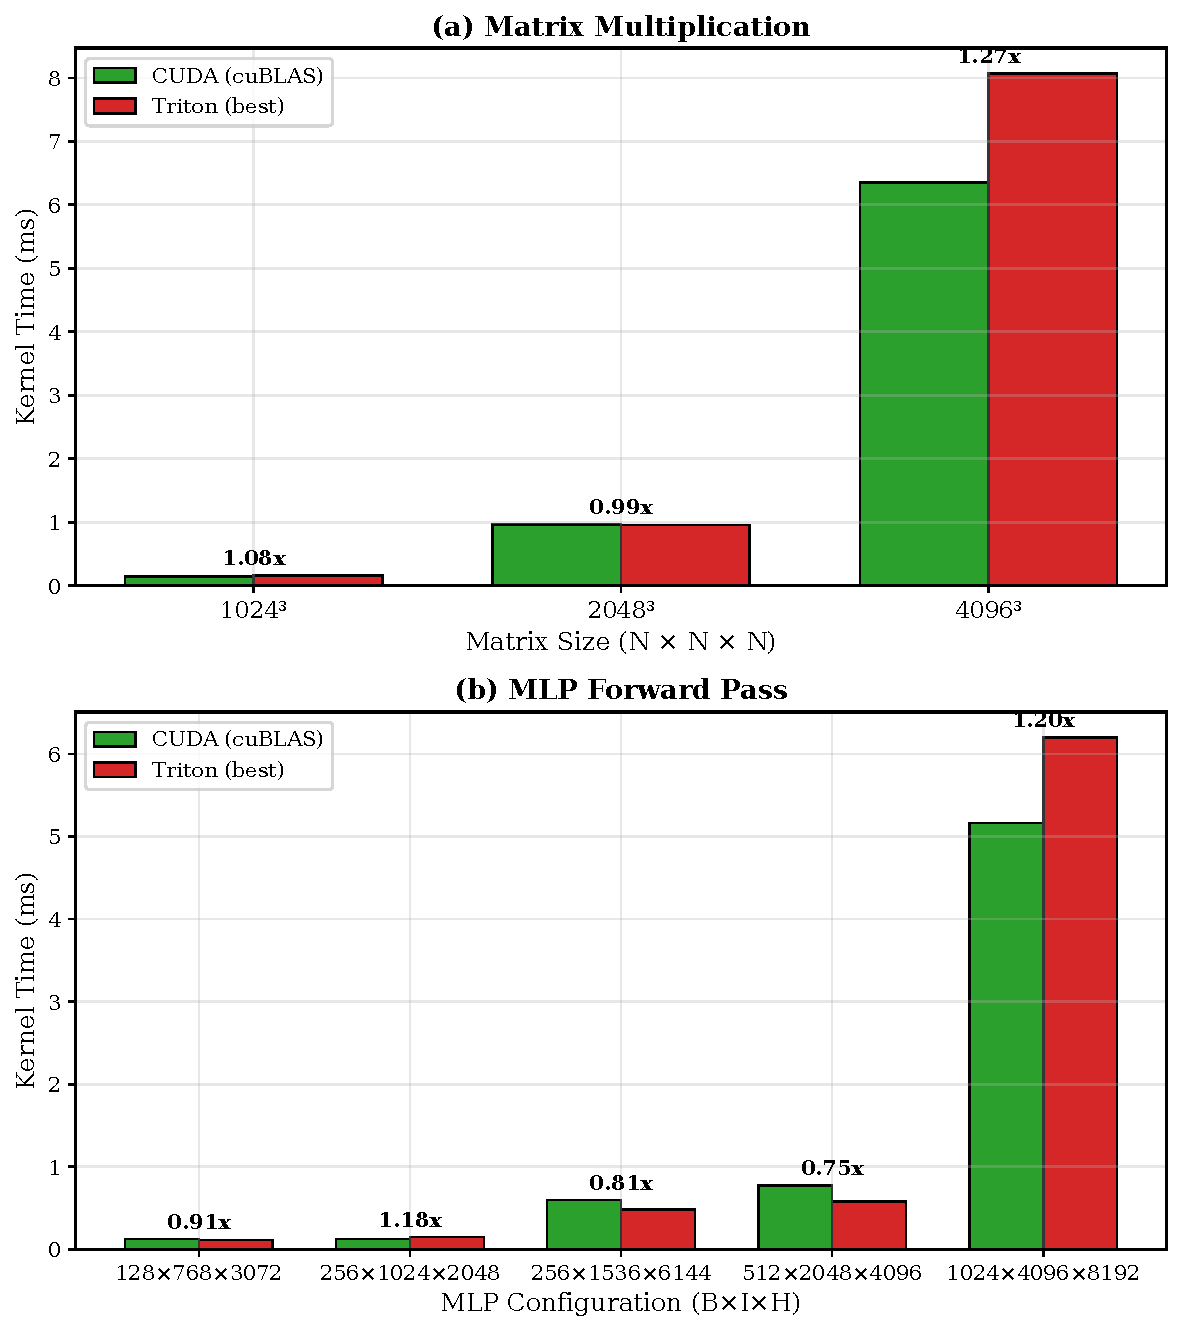
\includegraphics[width=\linewidth]{figures/fig_structured_parity.pdf}
    \caption{Structured Workloads. (a) Matrix Multiplication: Triton achieves $0.99\times$--$1.27\times$ vs cuBLAS. (b) MLP Forward Pass: Triton achieves $0.75\times$--$1.20\times$, with kernel fusion providing speedups on larger models.}
    \label{fig:structured}
\end{figure}

\subsection{Irregular Workloads: The Gap}

The scenario changes for Finite State Machines (FSM). Fig.~\ref{fig:fsm_gap} shows the performance gap on a logarithmic scale.

CUDA implementations outperform Triton by 10--30$\times$ (median: 10$\times$). This gap is structural:
\begin{itemize}
    \item \textbf{Latency-Bound:} FSM processing requires reading single bytes at random locations. Triton's \texttt{tl.load} fetches blocks, causing bus under-utilization.
    \item \textbf{Control Flow:} Triton handles conditionals via masking. CUDA skips unnecessary work with thread-local logic.
\end{itemize}

\begin{figure}[htbp]
    \centering
    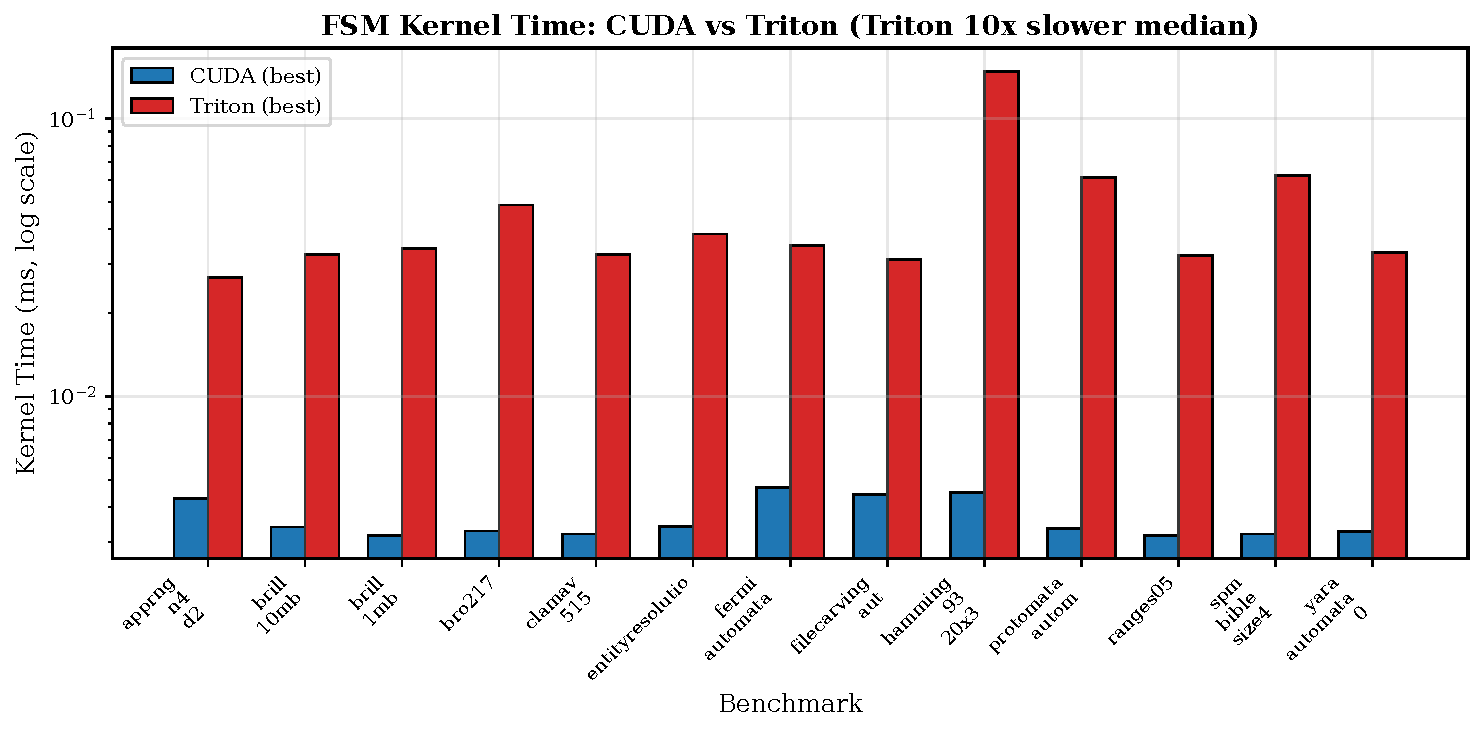
\includegraphics[width=\linewidth]{figures/fig_fsm_gap.pdf}
    \caption{The Irregularity Gap. CUDA kernels are 10--30$\times$ faster than Triton for FSM processing.}
    \label{fig:fsm_gap}
\end{figure}

\subsection{Technique Comparison: CUDA vs Triton}

Fig.~\ref{fig:cuda_techniques} compares FSM techniques from both CUDA and Triton across all benchmarks. CUDA techniques include Basic, CSR, ngAP, and BitGen. Triton techniques include DFS (best), CSR, and Bitmap.

\begin{figure*}[htbp]
    \centering
    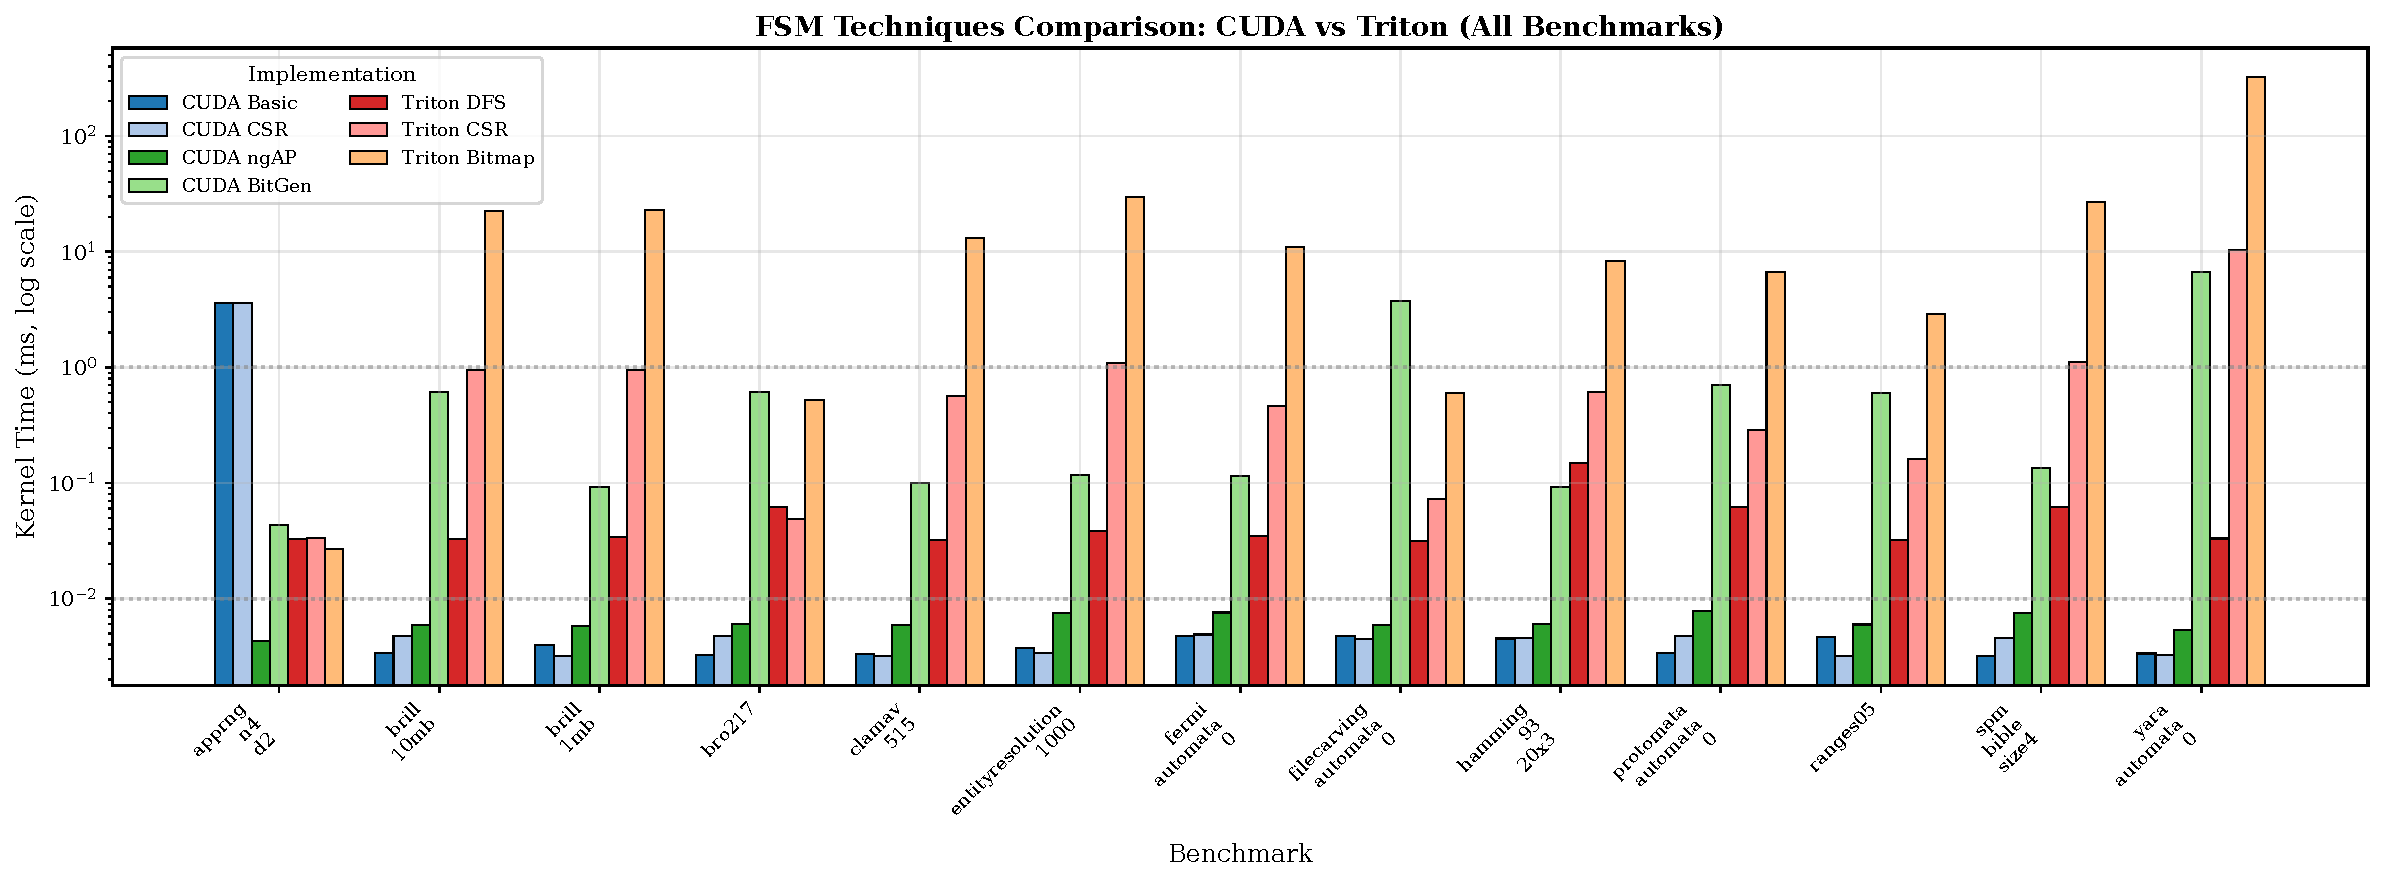
\includegraphics[width=\textwidth]{figures/fig_cuda_techniques.pdf}
    \caption{FSM Techniques Comparison: CUDA vs Triton. Blue/green bars show CUDA techniques (3--140~$\mu$s). Red/orange bars show Triton techniques (34~$\mu$s--15~ms). The gap is consistent across all benchmarks.}
    \label{fig:cuda_techniques}
\end{figure*}

Key findings:
\begin{itemize}
    \item \textbf{CUDA Basic/CSR:} Fastest overall (3--6~$\mu$s median). Simple serial traversal is effective when memory layout is optimized.
    \item \textbf{CUDA ngAP:} Comparable to Basic/CSR on single-stream workloads. ngAP~\cite{ngap} is designed for \emph{multi-stream} processing where thousands of input streams are processed in parallel. In our single-stream benchmark, the worklist overhead is not amortized.
    \item \textbf{CUDA BitGen:} Median 0.14~ms, slower than Basic for small inputs. BitGen~\cite{bitgen} transforms memory-bound workloads into compute-bound via bit-parallel operations. This approach benefits large-scale multi-pattern matching scenarios rather than single-stream processing.
    \item \textbf{Triton DFS:} Best Triton technique (34~$\mu$s median), but still $10\times$ slower than CUDA Basic.
    \item \textbf{Triton Bitmap:} Slowest approach (11--15~ms), $1000\times$ slower than CUDA Basic.
\end{itemize}

\textbf{Note on Advanced Techniques.} Both ngAP and BitGen are optimized for production scenarios with parallel input streams (e.g., network packet inspection processing thousands of packets simultaneously). Our single-stream benchmark favors simpler techniques. Production deployments should consider multi-stream batching where these advanced techniques may outperform Basic/CSR.

The gap between CUDA and Triton is consistent across all benchmarks and techniques, confirming the structural nature of the performance difference.

\subsection{Speedup Analysis}

Fig.~\ref{fig:speedup} shows the CUDA speedup over Triton for each FSM benchmark, sorted by magnitude. The speedup ranges from $6.2\times$ to $32.8\times$, with a median of $10.2\times$.

The benchmarks with highest speedup (brill, protomata, yara) involve complex automata with many states and transitions. The benchmarks with lower speedup (apprng, filecarving) have simpler structures where Triton's overhead is less pronounced.

\begin{figure}[htbp]
    \centering
    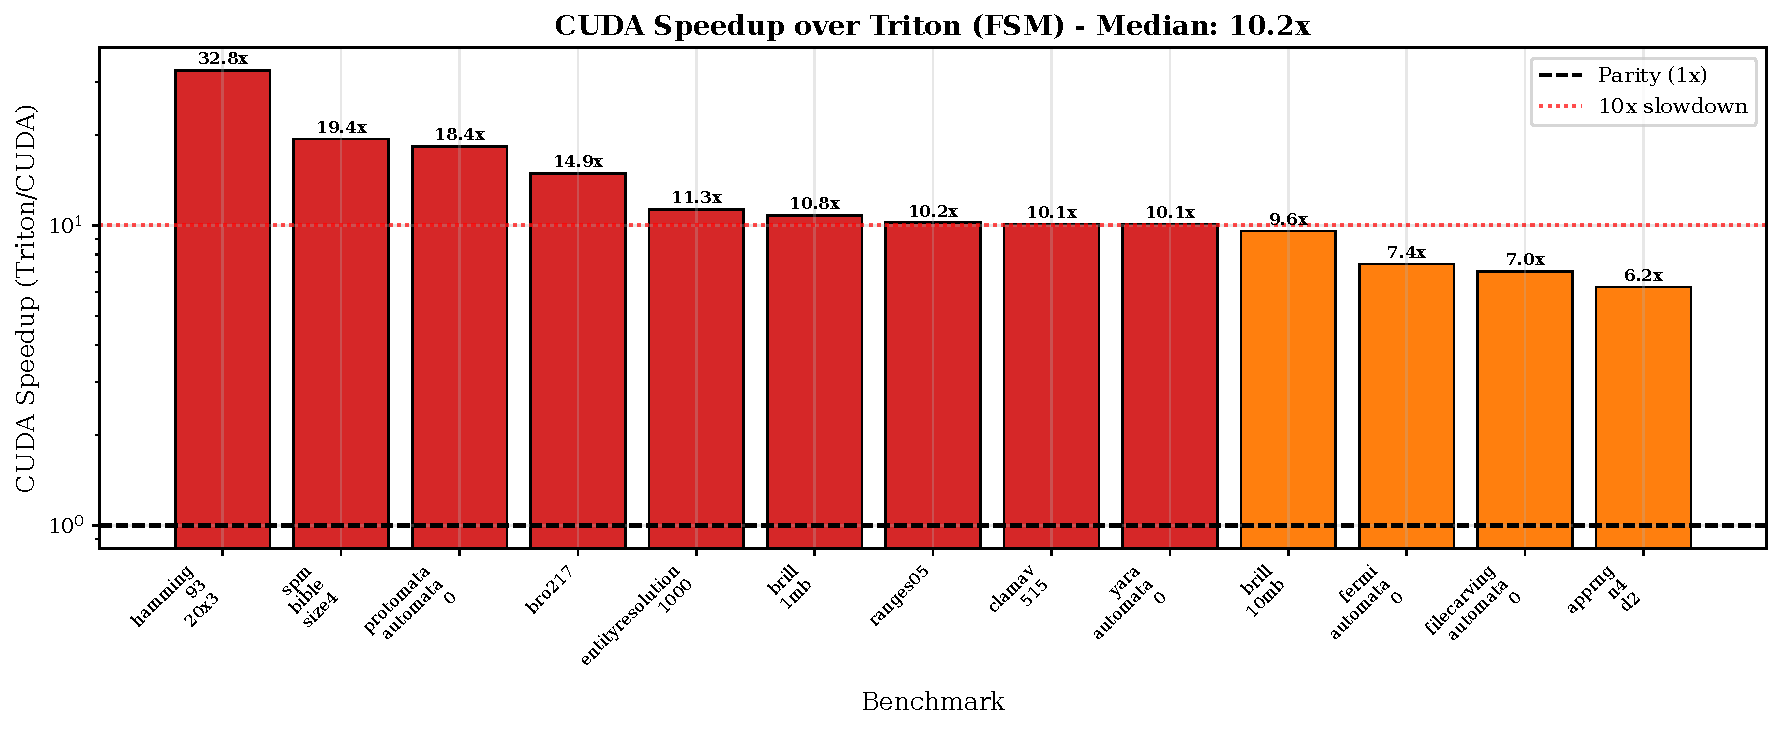
\includegraphics[width=\linewidth]{figures/fig_speedup_analysis.pdf}
    \caption{CUDA Speedup over Triton (FSM). Benchmarks sorted by speedup magnitude. Red bars indicate $>10\times$ slowdown, orange $5$--$10\times$, green $<5\times$.}
    \label{fig:speedup}
\end{figure}

\subsection{Productivity vs Performance Trade-off}

Fig.~\ref{fig:tradeoff} plots development effort (Lines of Code) against performance.

\begin{figure}[htbp]
    \centering
    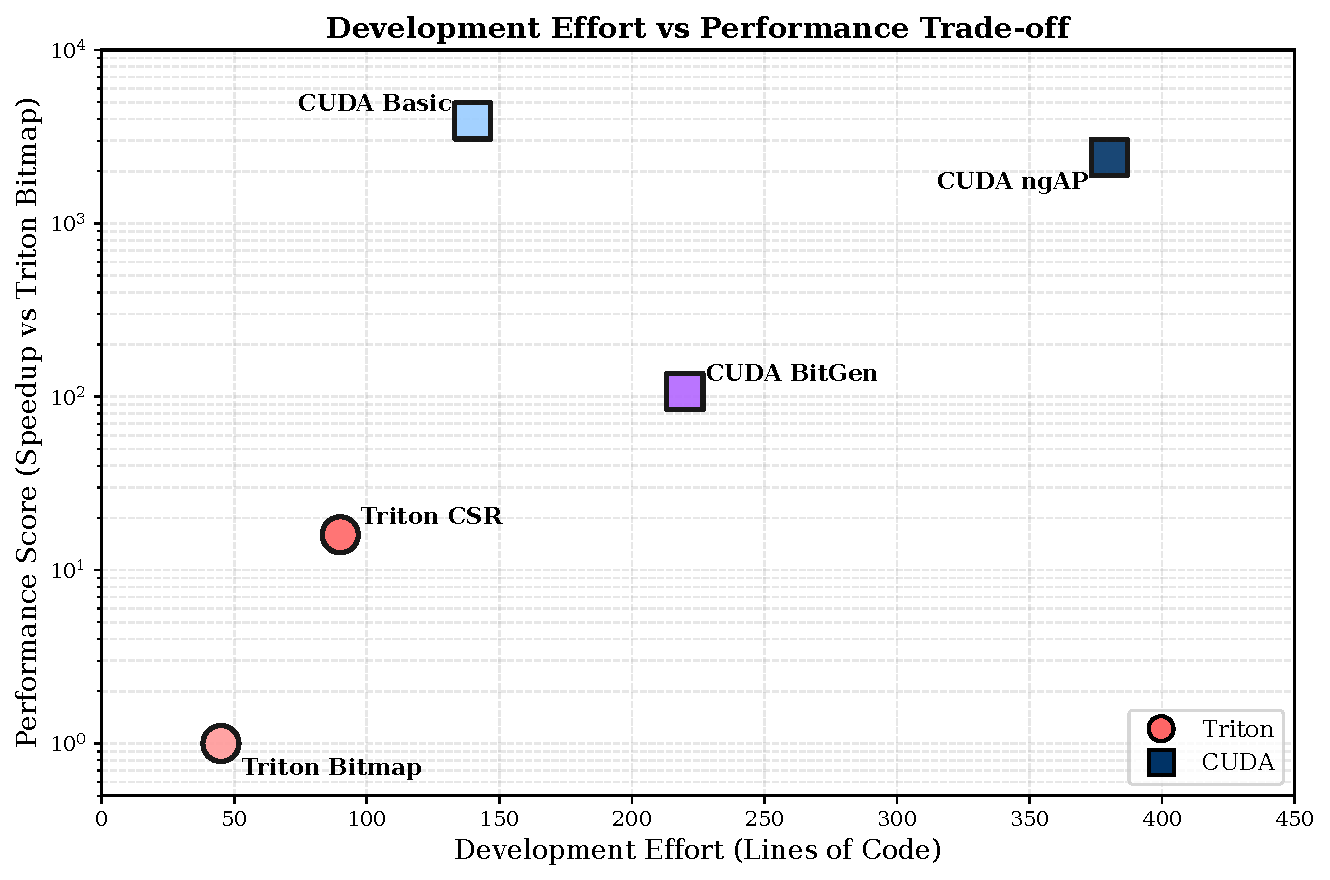
\includegraphics[width=\linewidth]{figures/fig_tradeoff.pdf}
    \caption{Productivity vs Performance. Triton allows concise code but hits a performance ceiling. CUDA techniques span a range of complexity and performance.}
    \label{fig:tradeoff}
\end{figure}

\begin{itemize}
    \item \textbf{Triton:} 45--60 LoC, lowest performance for FSM.
    \item \textbf{CUDA Basic/CSR:} 120--180 LoC, best performance for single-stream processing.
    \item \textbf{CUDA BitGen:} $\approx$250 LoC, competitive for multi-pattern workloads.
    \item \textbf{CUDA ngAP:} $\approx$380 LoC, complex implementation without proportional gains on our benchmark suite.
\end{itemize}

This demonstrates that for irregular workloads, the abstraction that makes Triton productive prevents expressing necessary low-level optimizations.

\subsection{System Overhead Analysis}

Fig.~\ref{fig:overhead} shows the breakdown between kernel execution time and system overhead (PCIe transfer, driver latency) for FSM workloads.

\begin{figure}[htbp]
    \centering
    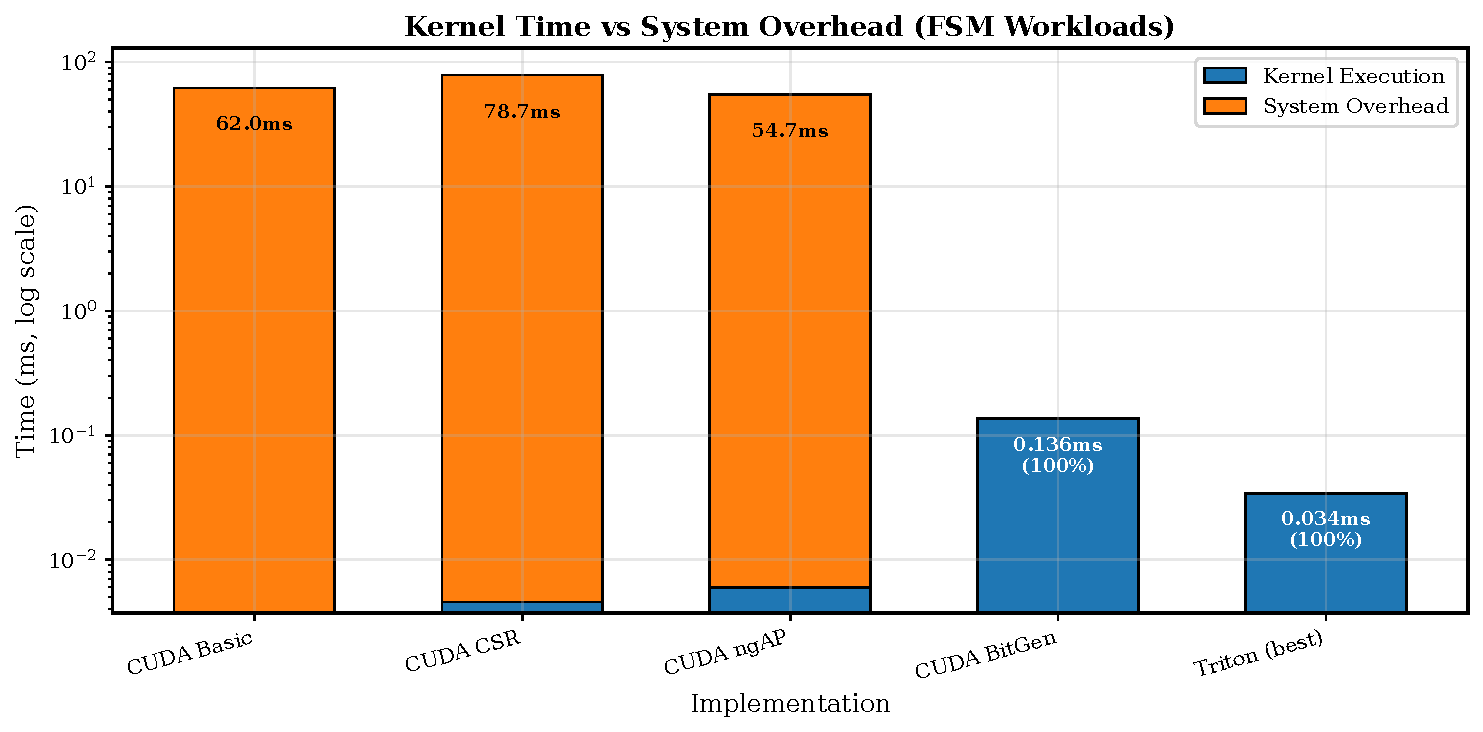
\includegraphics[width=\linewidth]{figures/fig_overhead.pdf}
    \caption{Kernel Time vs System Overhead. CUDA kernels are so fast (3--6~$\mu$s) that system overhead dominates total execution time.}
    \label{fig:overhead}
\end{figure}

For CUDA Basic/CSR, kernel execution represents less than 0.01\% of total time. The remaining 99.99\% is system overhead. This has important implications:
\begin{itemize}
    \item \textbf{Batching:} For production workloads, batching multiple FSM operations per kernel launch amortizes overhead.
    \item \textbf{Streaming:} Overlapping data transfer with computation can hide PCIe latency.
    \item \textbf{Triton advantage:} Triton's higher kernel time means overhead is proportionally smaller, making raw kernel comparisons misleading for end-to-end latency.
\end{itemize}
